\chapter{Kinematic Model of Non-holonomic omnidirectional mobile robot}
\label{cha:Kinematic}


\tikzset{
    wheel/.pic={
		\draw[gray, very thick] (-0.8,-0.1) rectangle (0.8,0.1);
		\filldraw [gray] (0,0) circle (1pt);
		\draw[->] (0,0) -- (1,0) node[anchor=north west] {$x^{wi}$};
		\draw[->] (0,0) -- (0,1) node[anchor=south east] {$y^{wi}$}; 
	}
};
\tikzset{
    platform/.pic={
		\filldraw [gray] (0,0) circle (2pt);
			\draw[thick,->] (0,0) -- (2,0) node[anchor=north west] {$x^b$};
			\draw[thick,->] (0,0) -- (0,2) node[anchor=south east] {$y^b$};
			\draw[thick,->] (0.75,0) arc (0:90:0.75) node[anchor=south west] {$\theta^b$};
			\draw[black, thick] (-4,-4) rectangle (4,4);
	}
};


Kinematics is the most basic study of how mechanical systems behave. In our case, Kinematics make a connection between joint states(driving rate, steering angle and steering velocity) and platform velocity in the 
task space. Which is fundmental for our control method.
First, a overview of the mobile platform is given (\cref{sec:model_overview}).
Afterwards, the Forward and Inverse Kinematic equations (\cref{sec:hum}) are presented.
%\cref{sec:application} explains how the model is implemented in different model predictive control (MPC) approaches.

\section{Model overview}
\label{sec:model_overview}

The the platform is a regid squre body with four conventional wheels on each corner. each wheel can be controlled independently (steering/driving).

In the task space, the frame is as shown in \cref{fig:taskSpace} we use $ \xi = [x,t,\theta]$ to discribe the current platform position and orientation, use $ \dot{\xi} = [\dot{x},\dot{y},\dot{\theta}] $ and 
$ \ddot{\xi}= [\ddot{x},\ddot{y},\ddot{\theta}] $ to discribe the platform velocity and acceleration. 

In the following discussion, we will mainly focus on to frames, world frame in which the odometry $ \hat{\xi} $ is calculated, and body frame in which the platform velocity $\hat{\dot{\xi}}^b$ and platform 
acceleration $ \hat{\ddot{\xi}}^b $ is calculated, the command from global planer $ \dot{\xi}^b $ and $ \ddot{\xi}^b $ is also assumed to be in the body frame. The lower case "b" in the upper corner indicates 
this variable is expressed in the body frame. While the notion with "hat" like $\hat{}$ is used to expressed the measured feedback.


\begin{figure}[t]
	\begin{center}
		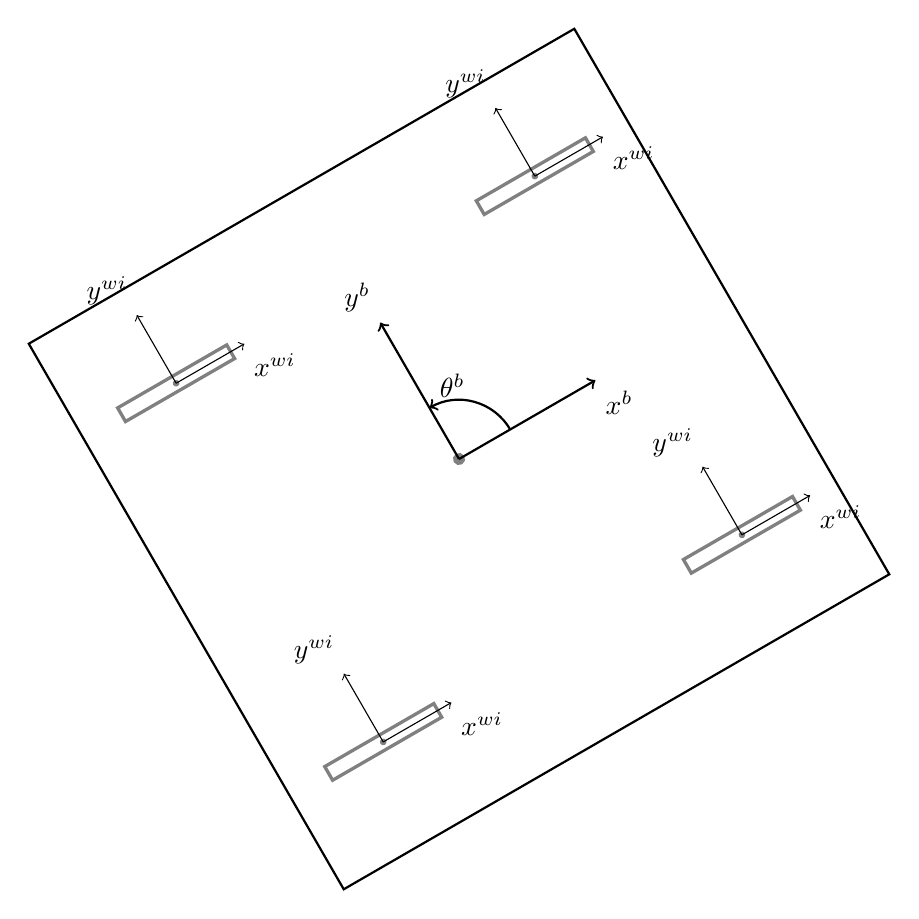
\begin{tikzpicture}[rotate=30 ]
			\pic[rotate=30 ] at(0,0) {platform};
			\pic[rotate=30 ] at(2.63,2.63) {wheel};
			\pic[rotate=30 ] at(2.63,-2.63) {wheel};
			\pic[rotate=30 ] at(-2.63,2.63) {wheel};
			\pic[rotate=30 ] at(-2.63,-2.63) {wheel};			
		\end{tikzpicture}
	\end{center}
\end{figure}



In the joint space we use $\beta_{i}$ and $\dot{\beta_{i}}$ to discribe the steering angle and steering velocity of the wheel, and $\dot{\phi}$ for driving velocity, which is shown in figure \cref{fig:wheel}. The measured
feedback from sensor is noted with $\hat{}$ while the joint space commands are without special notion. 

\begin{figure}[t]
\begin{center}
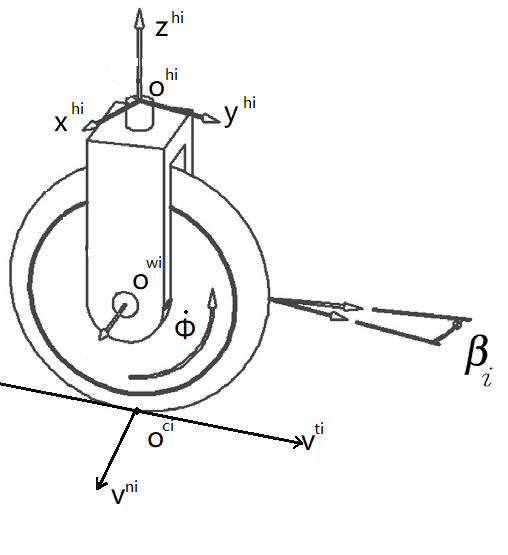
\includegraphics[width=.7\textwidth]{../Figures/wheel.png}
\caption{Wheel structure}
\label{fig:wheel}
\end{center}
\end{figure}




%%%%%%%%%%%%%%%%%%%%%%%%%%%%%%%%%%%%%%%%%%%%%%%%%%%%%%%%%%%%%%%%%%%%%%%%%%%%%
\section{Kinematics model}
\label{sec:Kinematics}
The Kinematic model is derived from the assumption that the wheels roll without slipping and there is no lateral skidding. The no-skidding constraint gurantee that there will be a unique instantaneous center of rotation(ICR) 
The ICR is term defined by Descartes' principle of instantaneous motion: 
\textit{At each instant, the motion of a planar rigid body coincides either with a pure translation, or with a pure rotation about some point, termed 
instantaneous center of rotation.}
Such feature distingushes this structure from the differential drive, gurantees the manuvior process to be quiet and robust.
We express the velocity of i-th wheel's contact point with ground by $V_{ci}=[v_{ti},v_{ni},0]$, where $v_{ti},v_{ni}$ respectively is the contact point's  tangential and normal velocitys. Which is illustrated in 
figure \cref{fig:contact_point}.



We can dirive the equation as follows:
\begin{equation}\label{eq:contact_point_velocity}
	\begin{split}
	V_{ci} &= T_b^{wi} [T_l^b\dot{\xi} + \dot{\theta}\overrightarrow{z_b}\times\overrightarrow{o_bo_{ci}} + \dot{\beta_i}T_{wi}^b\overrightarrow{z_{wi}}\times\overrightarrow{o_{wi}o_{ci}}] + \dot{\phi_i}\overrightarrow{x_{wi}}r_w
	\end{split}
\end{equation}

Where $T_b^w$,$T_l^b$ and $T_w^b$ are frame transfer matrix from body to wheel, from inertial to body and from wheel to body respectively. And $\overrightarrow{z_b}$, $\overrightarrow{z_w}$ and 
$\overrightarrow{x_w}$ are unit vectors along with positive direction of z axis of body frame, positive direction of z axis of wheel frame and positive direction of x axis of wheel frame.

With the above equation \cref{eq:contact_point_velocity} we can derive the contact point tangential velocity seprately
\begin{equation}\label{eq:contact_point_tangential}
	\begin{split}
	V_{ti} &= [cos(\beta_i), sin(\beta_i), -h_{yi}cos(\beta_i)+h_{xi}sin(\beta_i)]\dot{\xi^b} - r_w\dot{\phi_i}
	\end{split}
\end{equation}
And normal velocitys seprately.
\begin{equation}\label{eq:contact_point_normal}
	\begin{split}
	V_{ni} &= [-sin(\beta_i), cos(\beta_i), h_{xi}cos(\beta_i)+h_{yi}sin(\beta_i)]\xi^b
	\end{split}
\end{equation}

\subsection{Inverse Kinematics}
\label{sec:inverseKinematics}

To follow the constraints we defined in the begining, we set \cref{eq:contact_point_normal}$V_{ni}=0$. From which we can derive the expression of steering angles given the task space velocity command 
$\dot{\xi}=[\dot{x},\dot{y},\dot{\theta}]$.
\begin{equation}\label{eq:beta}
	\begin{split}
	\beta_i &= tan^{-1}(\frac{\dot{y^b}+h_{xi}\dot{\theta^b}}{\dot{x^b}-h_{yi}\dot{\theta^b}})
	\end{split}
\end{equation}

To express the steering velocity $\dot{\beta}$, we simplify the equation \cref{eq:contact_point_normal} by $V_{ni}=g(\dot{\beta_i})\dot{\xi^b}$ and differentiate it w.r.t. time:
\begin{equation}\label{eq:betaDot}
	\begin{split}
	\dot{\beta_i} &= \frac{-g(\dot{\beta_i})\ddot{\xi}}{\frac{dg(\dot{\beta_i})}{d\beta_i}\dot{\xi}}=\frac{\partial\beta_i}{\partial\dot{x}^b}\ddot{x}^b+\frac{\partial\beta_i}{\partial\dot{y}^b}\ddot{y}^b +\frac{\partial\beta_i}{\partial\dot{\theta^b}}\ddot{\theta}^b
	=f_{1i}(\dot{\xi^b})\ddot{\xi^b}
	\end{split}
\end{equation}

To express the driving rate of each wheel, we consider the constraint on tangential velocity, \cref{eq:contact_point_tangential} $V_{ti}=0 $ and we get:
\begin{equation}\label{eq:phi}
	\begin{split}
	\dot{\phi_i} &= \frac{1}{r_w}[cos(\beta_i), sin(\beta_i), -h_{yi}cos(\beta_i)+h_{xi}sin(\beta_i)]\dot{\xi^b}=f_{2i}(\beta)\dot{\xi^b}
	\end{split}
\end{equation}

Equation \cref{eq:beta},\cref{eq:betaDot} and \cref{eq:phi} illustrate the relationship between input velocity command in task space and the joint space response. By grouping them together, we get the Inverse Kinematics model


\subsection{Forward Kinematics}
\label{sec:forwardKinematics}

Similar to the process above, from \cref{eq:contact_point_tangential} we can also derive the forward Kinematic model, which takes the measured steering angle $\hat{\beta}$ driving velocity $\hat{\dot{\phi}}$ as input to 
calculate the platform current velocity $\hat{\dot{\xi}}$. For simplification, we simplify \cref{eq:contact_point_tangential}as $V_{fi}=f(\hat{\beta_i})\dot{\xi^b} -r_w\hat{\dot{\phi}}$
\begin{equation}
	\label{eq:forwardKinematics}
	\begin{split}
	\hat{\dot{\xi}} &= F^+(\hat{\beta})r_w\hat{\dot{\phi}},\\
	F(\hat{\beta}) &= [f(\hat{\beta_1})^T, f(\hat{\beta_2})^T, f(\hat{\beta_3})^T, f(\hat{\beta_4})^T]
	\end{split}
	\end{equation}
where $F^+(*)$ denotes pseudo inverse. One thing to be noticed is that classic psudo inverse will encountor singularities when platform has no rotation speed($\dot{\theta}=0$) where all 4 wheels are in parallel. In this case the $F(\hat{\beta})$matrix lose rank and the result would be inaccurate, we solve this by using the $pinv()$ function in Matlab and increase the singularity tolerance.

%%%%%%%%%%%%%%%%%%%%%%%%%%%%%%%%%%%%%%%%%%%%%%%%%%%%%%%%%%%%%%%%%%%%%%%%%%%%%%%%%%%%%%%%%%%%%%%%%%%%%%%%%%%%%%%%%%%%%%%%%%%%%%%%%%%%%%%%%%%%%%%%%%%%%%%%%%
%%%%%%%%%%%%%%%%%%%%%%%%%%%%%%%%%%%%%%%%%%%%%%%%%%%%%%%%%%%%%%%%%%%%%%%%%%%%%%%%%%%%%%%%%%%%%%%%%%%%%%%%%%%%%%%%%%%%%%%%%%%%%%%%%%%%%%%%%%%%%%%%%%%%%%%%%%

